\documentclass[aspectratio=169,10pt]{beamer}

\usetheme{default}
\usefonttheme{professionalfonts}
\setbeamertemplate{navigation symbols}{}
\setbeamersize{text margin left=0.75cm,text margin right=0.75cm}

\usepackage[T1]{fontenc}
\usepackage{array}
\usepackage{booktabs}
\usepackage{graphicx}
\usepackage{tikz}
\usepackage{xspace}
\usetikzlibrary{arrows.meta,positioning}

\definecolor{Ink}{HTML}{17212B}
\definecolor{Muted}{HTML}{66717D}
\definecolor{Paper}{HTML}{F7F9FA}
\definecolor{Line}{HTML}{D9E0E5}
\definecolor{Teal}{HTML}{087E8B}
\definecolor{TealLight}{HTML}{DCEFF0}
\definecolor{Coral}{HTML}{D95D39}
\definecolor{CoralLight}{HTML}{F8E4DE}
\definecolor{Gold}{HTML}{C58B13}
\definecolor{GoldLight}{HTML}{F6ECD2}
\definecolor{Green}{HTML}{2E7D5B}
\definecolor{GreenLight}{HTML}{DDEEE6}

\setbeamercolor{normal text}{fg=Ink,bg=white}
\setbeamercolor{frametitle}{fg=Ink}
\setbeamercolor{structure}{fg=Teal}
\setbeamercolor{itemize item}{fg=Teal}
\setbeamercolor{itemize subitem}{fg=Teal}
\setbeamerfont{frametitle}{size=\Large,series=\bfseries}
\setbeamerfont{footline}{size=\scriptsize}

\setbeamertemplate{frametitle}{
  \vspace{0.28cm}
  \insertframetitle\par
  \vspace{0.10cm}
  {\color{Teal}\rule{\linewidth}{0.7pt}}
}
\setbeamertemplate{footline}{
  \leavevmode
  \hbox to \paperwidth{%
    \hspace{0.75cm}%
    {\usebeamerfont{footline}\color{Muted}Amirhossein Bagheri}%
    \hfill
    {\usebeamerfont{footline}\color{Muted}Experimental Process
      \quad \insertframenumber/\inserttotalframenumber}%
    \hspace{0.42cm}%
  }
  \vspace{0.22cm}
}
\setbeamertemplate{itemize item}{\raise0.2ex\hbox{\small$\blacktriangleright$}}
\setbeamertemplate{itemize subitem}{\raise0.2ex\hbox{\scriptsize$\bullet$}}

\newcommand{\system}{\textsc{PMDS Forecasting Project}\xspace}
\newcommand{\key}[1]{{\color{Teal}\textbf{#1}}}
\newcommand{\tagbox}[2]{%
  \tikz[baseline=(tag.base)]{
    \node[fill=#1,rounded corners=1.5pt,inner xsep=6pt,inner ysep=3pt]
      (tag) {\strut #2};
  }%
}
\newcolumntype{L}[1]{>{\raggedright\arraybackslash}p{#1}}
\newcolumntype{C}[1]{>{\centering\arraybackslash}p{#1}}

\title{\system: Experimental Process}
\author{Amirhossein Bagheri}
\institute{Politecnico di Milano \qquad Supervisor: Tommaso Bianchi}
\date{}

\begin{document}
\section{Experimental Process}

% ------------------------------------------------------------
\begin{frame}[plain]
  \vspace{0.55cm}
  {\color{Teal}\rule{1.25cm}{3pt}}

  \vspace{0.48cm}
  {\fontsize{27}{32}\selectfont\bfseries Experimental Process\par}

  \vspace{0.35cm}
  {\Large\color{Muted}
    Clean-data evaluation, reproducible execution,\
    and traceable result consolidation\par}

  \vspace{0.62cm}
  \begin{center}
    \begin{minipage}{0.88\linewidth}
      \large\raggedright
      The experiment compared \key{time-series foundation models} with
      \key{established forecasting baselines} under one consistent
      clean-data evaluation pipeline.
    \end{minipage}
  \end{center}

  \vfill
  \tagbox{TealLight}{\small\textbf{12 datasets}}
  \hspace{0.18cm}
  \tagbox{GreenLight}{\small\textbf{Rolling-origin evaluation}}
  \hspace{0.18cm}
  \tagbox{GoldLight}{\small\textbf{Four consolidated artifacts}}
\end{frame}

% ------------------------------------------------------------
\begin{frame}{Dataset portfolio: 12 clean evaluation datasets}
  \vspace{0.10cm}
  \begin{columns}[T,totalwidth=0.94\linewidth]
    \begin{column}{0.44\linewidth}
      \tagbox{TealLight}{\textbf{Chronos / Monash datasets}}

      \vspace{0.24cm}
      \begin{itemize}
        \item M1 Yearly
        \item M4 Hourly
        \item Weather
        \item M3 Quarterly
        \item Car Parts
        \item NN5 Weekly
      \end{itemize}
    \end{column}

    \begin{column}{0.44\linewidth}
      \tagbox{GoldLight}{\textbf{External datasets}}

      \vspace{0.24cm}
      \begin{itemize}
        \item National Illness
        \item Traffic
        \item PSM
        \item Elexon Electricity Demand
        \item USGS Streamflow
        \item BLS Macroeconomic Indicators
      \end{itemize}
    \end{column}
  \end{columns}

  \vspace{0.30cm}
  \centering
  \tagbox{GreenLight}{\small Six benchmark datasets \quad + \quad six external datasets}
\end{frame}

% ------------------------------------------------------------
\begin{frame}{External-data provenance and reproducibility}
  \vspace{0.12cm}
  \begin{columns}[T,totalwidth=0.94\linewidth]
    \begin{column}{0.43\linewidth}
      \tagbox{CoralLight}{\textbf{Credential-dependent sources}}

      \vspace{0.24cm}
      \begin{itemize}
        \item EIA-930 required an API credential.
        \item FRED-MD required an API credential.
        \item Both were excluded from the clean benchmark.
      \end{itemize}
    \end{column}

    \begin{column}{0.43\linewidth}
      \tagbox{GreenLight}{\textbf{Keyless official sources}}

      \vspace{0.24cm}
      \begin{itemize}
        \item Elexon demand was added as a replacement.
        \item BLS indicators were added as a replacement.
        \item USGS streamflow was retained as a credential-free source.
      \end{itemize}
    \end{column}
  \end{columns}

  \vspace{0.42cm}
  \begin{center}
    \begin{minipage}{0.86\linewidth}
      \large\raggedright
      Official external observations were normalized and stored as
      \key{reproducible local snapshots}. Subsequent runs reused the same
      timestamped values and verified snapshot integrity.
    \end{minipage}
  \end{center}
\end{frame}

% ------------------------------------------------------------
\begin{frame}{Original clean model comparison}
  \vspace{0.10cm}
  \begin{columns}[T,totalwidth=0.95\linewidth]
    \begin{column}{0.44\linewidth}
      \tagbox{TealLight}{\textbf{Three foundation models}}

      \vspace{0.26cm}
      \begin{itemize}
        \item Amazon Chronos T5 Tiny
        \item Google TimesFM 2.5 200M
        \item Salesforce Moirai 2.0 Small
      \end{itemize}
    \end{column}

    \begin{column}{0.44\linewidth}
      \tagbox{GoldLight}{\textbf{Five comparison models}}

      \vspace{0.26cm}
      \begin{itemize}
        \item ARIMA(2,1,2)
        \item AutoARIMA
        \item Prophet
        \item DeepAR
        \item Seasonal Naive
      \end{itemize}
    \end{column}
  \end{columns}

  \vspace{0.55cm}
  \centering
  \tagbox{GreenLight}{\small Common tasks, forecast horizons, quantiles, and metric implementation}
\end{frame}

% ------------------------------------------------------------
\begin{frame}{Separate Chronos checkpoint-scale experiment}
  \vspace{0.08cm}
  \begin{columns}[T,totalwidth=0.95\linewidth]
    \begin{column}{0.53\linewidth}
      \small
      \renewcommand{\arraystretch}{1.28}
      \setlength{\tabcolsep}{5pt}
      \begin{tabular}{L{0.60\linewidth} C{0.25\linewidth}}
        \toprule
        \textbf{Checkpoint} & \textbf{Parameters} \\
        \midrule
        Chronos T5 Mini  & $\sim$20M \\
        Chronos T5 Small & $\sim$46M \\
        Chronos T5 Base  & $\sim$200M \\
        Chronos T5 Large & $\sim$710M \\
        \bottomrule
      \end{tabular}
    \end{column}

    \begin{column}{0.37\linewidth}
      \scriptsize
      \tagbox{GreenLight}{\textbf{Execution settings}}

      \vspace{0.20cm}
      \begin{itemize}
        \item All 12 datasets
        \item GPU execution
        \item bfloat16 inference
        \item Three repetitions per stochastic forecast
        \item 100 forecast samples per repetition
      \end{itemize}
    \end{column}
  \end{columns}

  \vspace{0.38cm}
  \centering
  \tagbox{TealLight}{\small All 12 datasets completed with zero failed model tasks}
\end{frame}

% ------------------------------------------------------------
\begin{frame}{Evaluation procedure: tasks and forecast outputs}
  \vspace{0.06cm}
  \begin{columns}[T,totalwidth=0.96\linewidth]
    \begin{column}{0.45\linewidth}
      \tagbox{TealLight}{\textbf{Task construction}}

      \vspace{0.20cm}
      \scriptsize
      \begin{itemize}
        \item Maximum historical context: 512 observations
        \item Dataset-specific horizons and seasonalities
        \item Multiple rolling forecast origins
        \item Generally three origins per selected series
        \item Two origins for Car Parts
        \item Task totals varied with eligible series and origins
      \end{itemize}
    \end{column}

    \begin{column}{0.43\linewidth}
      \tagbox{GoldLight}{\textbf{Forecast representation}}

      \vspace{0.20cm}
      \scriptsize
      \begin{itemize}
        \item Median used as the point forecast
        \item Quantiles from 0.1 through 0.9
        \item MAE, RMSE, sMAPE, MASE, and weighted quantile loss
        \item Rain occurrence error where applicable
        \item Positive-value MAE where applicable
      \end{itemize}
    \end{column}
  \end{columns}
\end{frame}

% ------------------------------------------------------------
\begin{frame}{Evaluation procedure: reproducibility record}
  \vspace{0.18cm}
  \begin{center}
    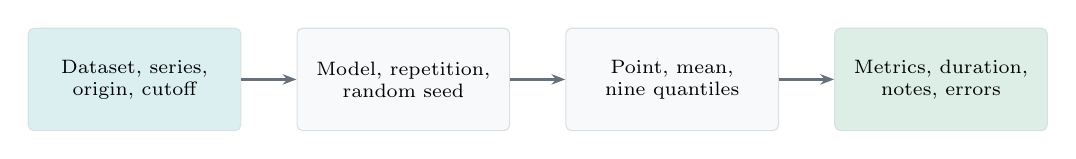
\begin{tikzpicture}[
      node distance=7mm,
      box/.style={draw=Line,fill=Paper,rounded corners=2pt,align=center,
        minimum width=27mm,minimum height=13mm,font=\scriptsize},
      arrow/.style={-{Stealth[length=5pt]},thick,color=Muted}
    ]
      \node[box,fill=TealLight] (task) {Dataset, series,\\origin, cutoff};
      \node[box,right=of task] (run) {Model, repetition,\\random seed};
      \node[box,right=of run] (forecast) {Point, mean,\\nine quantiles};
      \node[box,right=of forecast,fill=GreenLight] (record) {Metrics, duration,\\notes, errors};
      \draw[arrow] (task) -- (run);
      \draw[arrow] (run) -- (forecast);
      \draw[arrow] (forecast) -- (record);
    \end{tikzpicture}
  \end{center}

  \vspace{0.55cm}
  \begin{columns}[T,totalwidth=0.90\linewidth]
    \begin{column}{0.42\linewidth}
      \small
      \tagbox{GoldLight}{\textbf{Forecast horizon}}

      \vspace{0.18cm}
      Actual observations, point and mean forecasts, and all requested
      quantiles were retained at every timestamp.
    \end{column}
    \begin{column}{0.42\linewidth}
      \small
      \tagbox{TealLight}{\textbf{Historical context}}

      \vspace{0.18cm}
      Pre-cutoff observations were retained so trajectories can be plotted
      without rerunning any model.
    \end{column}
  \end{columns}
\end{frame}

% ------------------------------------------------------------
\begin{frame}{Three clean run groups}
  \vspace{0.12cm}
  \begin{center}
    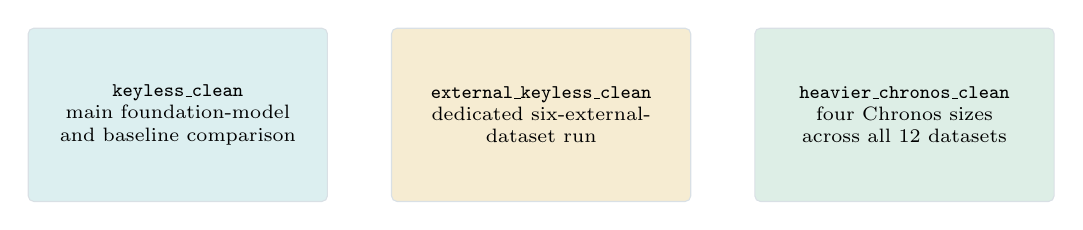
\begin{tikzpicture}[
      node distance=8mm,
      run/.style={draw=Line,rounded corners=2pt,align=center,
        minimum width=38mm,minimum height=22mm,font=\scriptsize},
      arrow/.style={-{Stealth[length=5pt]},thick,color=Muted}
    ]
      \node[run,fill=TealLight] (keyless)
        {\texttt{keyless\_clean}\\main foundation-model\\and baseline comparison};
      \node[run,fill=GoldLight,right=of keyless] (external)
        {\texttt{external\_keyless\_clean}\\dedicated six-external-\\dataset run};
      \node[run,fill=GreenLight,right=of external] (heavy)
        {\texttt{heavier\_chronos\_clean}\\four Chronos sizes\\across all 12 datasets};
    \end{tikzpicture}
  \end{center}

  \vspace{0.58cm}
  \begin{columns}[T,totalwidth=0.90\linewidth]
    \begin{column}{0.42\linewidth}
      \tagbox{CoralLight}{\small\textbf{Robustness experiment}}

      \vspace{0.15cm}
      \small Stopped by request and not included in the final clean results.
    \end{column}
    \begin{column}{0.42\linewidth}
      \tagbox{CoralLight}{\small\textbf{Forecast audit}}

      \vspace{0.15cm}
      \small Maintained separately and excluded from final consolidation.
    \end{column}
  \end{columns}
\end{frame}

% ------------------------------------------------------------
\begin{frame}{Final result consolidation}
  \vspace{-0.02cm}
  \begin{center}
    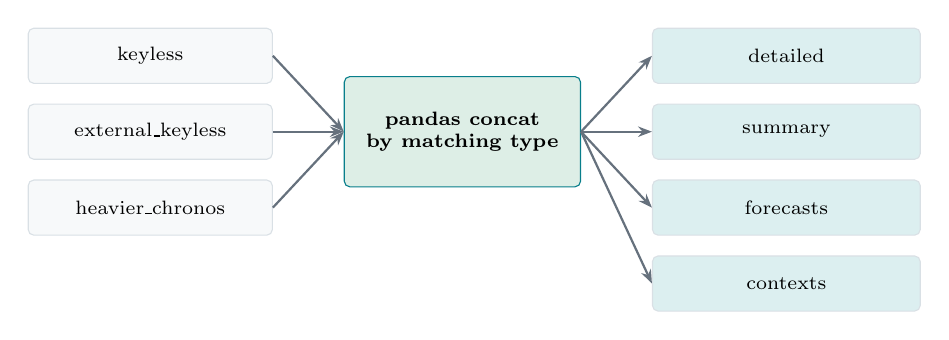
\begin{tikzpicture}[
      node distance=2.5mm and 8mm,
      source/.style={draw=Line,fill=Paper,rounded corners=2pt,align=center,
        minimum width=31mm,minimum height=7mm,font=\scriptsize},
      merge/.style={draw=Teal,fill=GreenLight,rounded corners=2pt,align=center,
        minimum width=30mm,minimum height=14mm,font=\scriptsize\bfseries},
      artifact/.style={draw=Line,fill=TealLight,rounded corners=2pt,align=center,
        minimum width=34mm,minimum height=7mm,font=\scriptsize},
      arrow/.style={-{Stealth[length=5pt]},thick,color=Muted}
    ]
      \node[source] (k) {keyless};
      \node[source,below=of k] (e) {external\_keyless};
      \node[source,below=of e] (h) {heavier\_chronos};
      \node[merge,right=9mm of e] (merge) {pandas concat\\by matching type};
      \node[artifact,right=9mm of merge] (s) {summary};
      \node[artifact,above=of s] (d) {detailed};
      \node[artifact,below=of s] (f) {forecasts};
      \node[artifact,below=of f] (c) {contexts};
      \draw[arrow] (k.east) -- (merge.west);
      \draw[arrow] (e.east) -- (merge.west);
      \draw[arrow] (h.east) -- (merge.west);
      \draw[arrow] (merge.east) -- (d.west);
      \draw[arrow] (merge.east) -- (s.west);
      \draw[arrow] (merge.east) -- (f.west);
      \draw[arrow] (merge.east) -- (c.west);
    \end{tikzpicture}
  \end{center}

  \vspace{0.02cm}
  \scriptsize
  \begin{itemize}
    \setlength{\itemsep}{1pt}
    \item Matching CSV types were concatenated with pandas.
    \item Artifact types remained separate because they represent different experimental levels.
    \item Every final row received a \texttt{source\_run} value.
    \item Rows were preserved without deduplication so overlapping runs remain traceable.
    \item Final row counts were checked against all contributing source CSVs.
  \end{itemize}
\end{frame}

% ------------------------------------------------------------
\begin{frame}{Consolidated artifacts: task- and dataset-level records}
  \vspace{0.10cm}
  \begin{columns}[T,totalwidth=0.95\linewidth]
    \begin{column}{0.44\linewidth}
      \tagbox{TealLight}{\textbf{Detailed --- 10,502 rows}}

      \vspace{0.20cm}
      \scriptsize
      One record per model repetition and forecasting task:
      \begin{itemize}
        \item dataset, series, origin, and cutoff
        \item model, repetition, and random seed
        \item forecast-distribution type and metrics
        \item duration, diagnostic notes, and errors
      \end{itemize}

      \vspace{0.10cm}
      \texttt{final\_clean\_detailed.csv}
    \end{column}

    \begin{column}{0.44\linewidth}
      \tagbox{GoldLight}{\textbf{Summary --- 176 rows}}

      \vspace{0.20cm}
      \scriptsize
      One aggregate record per dataset--model combination:
      \begin{itemize}
        \item aggregate metric fields
        \item evaluated, successful, and failed tasks
        \item successful and failed runs
        \item diagnostic status and total duration
      \end{itemize}

      \vspace{0.10cm}
      \texttt{final\_clean\_summary.csv}
    \end{column}
  \end{columns}
\end{frame}

% ------------------------------------------------------------
\begin{frame}{Consolidated artifacts: timestamp-level records}
  \vspace{0.10cm}
  \begin{columns}[T,totalwidth=0.95\linewidth]
    \begin{column}{0.44\linewidth}
      \tagbox{GreenLight}{\textbf{Forecasts --- 208,104 rows}}

      \vspace{0.20cm}
      \scriptsize
      Timestamp-level forecast outputs:
      \begin{itemize}
        \item dataset, series, origin, model, and repetition
        \item seed, forecast step, and timestamp
        \item actual, point forecast, and mean forecast
        \item quantiles from 0.1 through 0.9
      \end{itemize}

      \vspace{0.10cm}
      \texttt{final\_clean\_forecasts.csv}
    \end{column}

    \begin{column}{0.44\linewidth}
      \tagbox{TealLight}{\textbf{Contexts --- 72,682 rows}}

      \vspace{0.20cm}
      \scriptsize
      Historical observations supplied before each cutoff:
      \begin{itemize}
        \item dataset, series, and rolling origin
        \item historical step and timestamp
        \item observed value
        \item joins with forecasts for full trajectory plots
      \end{itemize}

      \vspace{0.10cm}
      \texttt{final\_clean\_contexts.csv}
    \end{column}
  \end{columns}

  \vspace{0.36cm}
  \centering
  \tagbox{GoldLight}{\small\texttt{source\_run}: keyless \quad | \quad external\_keyless \quad | \quad heavier\_chronos}
\end{frame}

\end{document}
